\chapter{研究方法與實作}
本章節將詳述如何針對i18n工具現存的四項問題,進行思考與改善,並與朱峻平的論文“支援多國語言的Robot Framework網頁自動化驗收測試” (第一版i18n工具)進行比較,呈現出先後的差異。

\section{系統設計}
i18n系統類別圖(如圖3.1),沿用自第一版i18n工具的架構,經過部分實作的改善,並且新增了一個用於顯示一詞多譯選項的圖形化使用者介面類別(UI),以及20種代理關鍵字的類別。 

\begin{figure}[H]
\flushleft
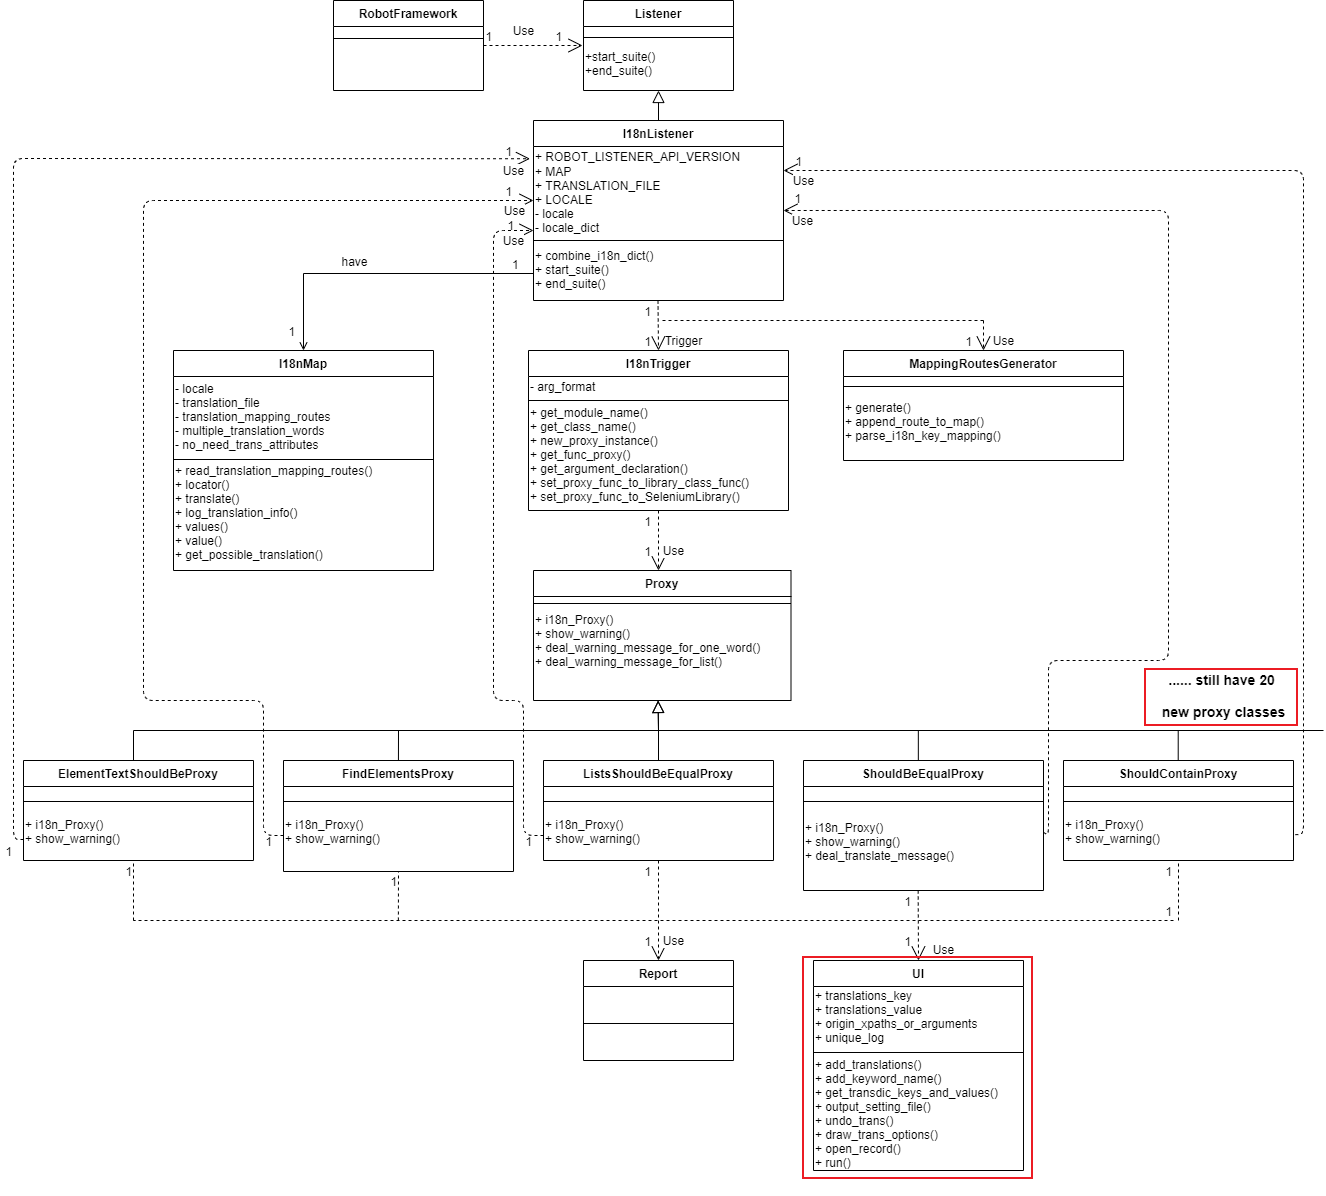
\includegraphics[width= 180mm]{../UML/i18n class diagram-i18n class diagram.png}
\caption{i18n系統類別圖}
\end{figure}

\hspace*{\fill} \\
\\ \hspace*{\fill} \\
\\ \hspace*{\fill} \\
\\ \hspace*{\fill} \\
\\ \hspace*{\fill} \\

以下將分別簡介本論文使用到的Robot Framework的原生類別、第一版i18n已存在的類別,以及本論文新增的類別。

\subsection{第一版i18n工具的現存類別與原生類別}
Robot Framework的原生類別分別有RobotFramework,Listener,和Report。
第一版i18n設計的類別則有I18nListener、MappingRoutesGenerator、I18nMap、I18nTrigger、Proxy,以及5個繼承自Proxy \cite{proxy} 的代理關鍵字類別: ShouldContainProxy、ElementTextShouldBeProxy、FindElementProxy、ListsShouldBeEqualProxy、ShouldBeEqualProxy。(詳請參考朱峻平的論文3-1)

 \hspace*{\fill} \\
\\ \hspace*{\fill} \\
\\ \hspace*{\fill} \\
\\ \hspace*{\fill} \\
\\ \hspace*{\fill} \\
\subsection{本論文新擴充的類別}
本論文新增的UI類別,其會在程式執行期間,記錄下遭遇到一詞多譯的詞語以及其翻譯。在程式執行後,產生一詞多譯的圖形化使用者介面,使用者選擇並提交希望的翻譯後,便會產生一個系統設定檔記錄翻譯選擇。
而其他20種新增的代理關鍵字類別(如表3.1),皆繼承自父類別Proxy並改寫其實作,負責代理各自對應關鍵字的參數部分翻譯,並將翻譯好的參數部分回傳給原關鍵字。
\hspace*{\fill} \\

\begin{table}[H]
    \centering
        \begin{tabular}{|l|l|}
        \hline
        \multicolumn{2}{|c|}{新增的代理關鍵字類别} \\ \hline
        1. AlertShouldBePresentProxy & 11. ListShouldNotContainDuplicatesProxy\\ 
        2. CountValuesInListProxy & 12. RemoveFromDictionaryProxy\\ 
        3. DictionariesShouldBeEqualProxy & 13. RemoveValuesFromListProxy\\
        4. DictionaryShouldContainItemProxy & 14. SelectFromListByLabelProxy\\
        5. DictionaryShouldContainKeyProxy & 15. SelectFromListByValueProxy\\
        6. DictionaryShouldContainValueProxy & 16. TableCellShouldContainProxy\\
        7. GetMatchCountProxy & 17. TableColumnShouldContainProxy\\
        8. ListSelectionShouldBeProxy & 18. TableRowShouldContainProxy\\
        9. ListShouldContainSubListProxy & 19. TableShouldContainProxy\\
        10. ListShouldContainValueProxy & 20. TitleShouldBeProxy\\   
        \hline
        \end{tabular}
    \caption{本論文新增的20種代理關鍵字類別}
\end{table}

\hspace*{\fill} \\
\subsection{系統執行流程}
在使用此i18n工具執行測試腳本前,首先使用者必須於Red編輯器\cite{red}中的Additional Robot Framework arguments設定系統參數(如圖3.2),設定為-d out –L debug -–listener i18n/listeners/I18nListener.py:zh-TW。

\begin{figure}[H]
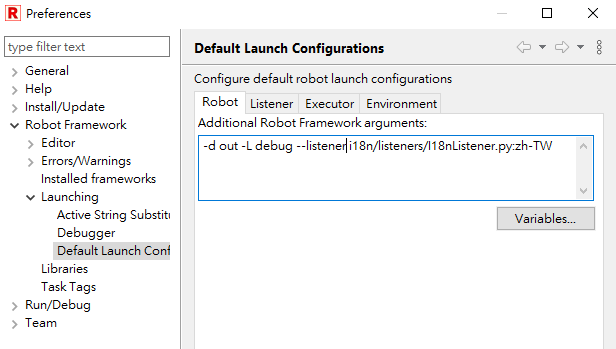
\includegraphics[width= 1.1\textwidth]{../論文截圖/3-1-3-1 設定系統參數.png}
\caption{Robot Framework系統參數設定}
\end{figure}

測試腳本執行時,系統會先去呼叫I18nListener.py並執行其實作,zh-TW代表當前語言為繁體中文-台灣。之後讀取由使用者自行提供的JSON格式翻譯檔(圖3.3),建立出一份“Key階層”對應“翻譯”的翻譯路徑檔(圖3.4),以及建立出所有自定義的代理關鍵字物件。每當腳本運行到一個有定義代理之關鍵字,系統就會去呼叫對應的代理關鍵字物件,並執行翻譯邏輯。

\begin{figure}[H]
\centering
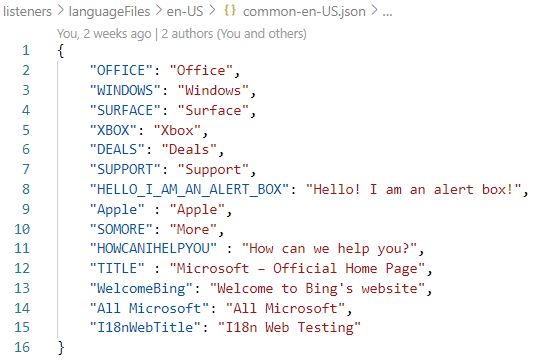
\includegraphics[width= .8\textwidth]{../論文截圖/3-1-3-2 JSON格式翻譯檔.png}
\caption{JSON格式翻譯檔}
\end{figure}
\begin{figure}[H]
\centering
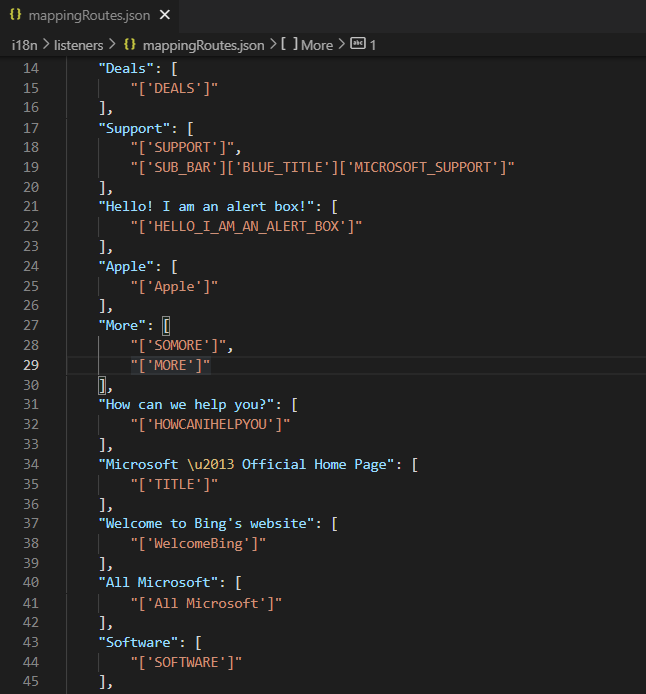
\includegraphics[width= .8\textwidth]{../論文截圖/3-1-3-3 翻譯路徑檔.png}
\caption{翻譯路徑檔示例}
\end{figure}

系統流程相較於第一版i18n改動較大的部份,是在測試腳本結束後。除了將一詞多譯的warning資訊顯示在報表上外,若是遭遇過一詞多譯,便會跳出一詞多譯的UI(詳見章節3-4),其記錄了執行翻譯當下關鍵字的參數組合,並顯示所有可能的翻譯詞,讓使用者可以從中去選擇並產生一個設定檔。之後再次執行測試腳本時,系統便會根據設定檔的內容去選擇適當的翻譯詞,同時消除報表上的warning提示資訊。

\hspace*{\fill} \\
\\ \hspace*{\fill} \\
\\ \hspace*{\fill} \\
\\ \hspace*{\fill} \\
\\ \hspace*{\fill} \\
\\ \hspace*{\fill} \\
\\ \hspace*{\fill} \\
%3.2
\section{擴充與修改代理關鍵字實作}
在此前,第一版i18n工具只支援7種Robot Framework原生關鍵字(如表3.2)。尚有31種參數部分需要翻譯的原生關鍵字,未提供支援。如果測試腳本使用到這些未支援的原生關鍵字去跑多國語言網頁測試,則會導致出錯。因此,本論文的解法是擴充完目前Robot Framework版本剩下的代理關鍵字,使得所有原生關鍵字的參數部分都能正確得被翻譯。

\renewcommand\arraystretch{0.8}
\begin{table}[H]
    \centering
    \setlength{\tabcolsep}{10mm}{
        \begin{tabular}{|l|}
        \hline
        第一版i18n已提供代理的關鍵字 \\
        \hline
        1. find\_element \\
        2. element\_text\_should\_be \\
        3. lists\_should\_be\_equal\\
        4. should\_be\_equal\\
        5. should\_not\_be\_equal\\
        6. should\_contain\\
        7. should\_not\_contain\\       
        \hline
        \end{tabular}}
    \caption{第一版i18n已提供代理的Robot Framework原生關鍵字}
\end{table}

且又因為先前的i18n工具分別在Robot Framework版本3.0.4、SeleniumLibrary版本3.1.1下開發,而現在的Robot Framework版本已更新到3.2.2,SeleniumLibrary版本則更新到4.5.0,導致原先需要被支援的31種原生關鍵字,有兩種已被淘汰:
input\_text\_into\_prompt、xpath\_should\_match\_x\_times。因此,還有29種原生關鍵字需要提供代理(如表3.3)。(‘*’標示為因版本更新導致被淘汰的原生關鍵字)

\begin{table}[H]
    \centering 
    \setlength{\tabcolsep}{5mm}{
        \begin{tabular}{|l|l|}
        \hline
        \multicolumn{2}{|c|}{待擴充的代理關鍵字}\\ \hline
        Collections Libaray (3.0.4) & SeleniumLibrary (4.5.0) \\ \hline
        1. count\_values\_in\_list & 1. alert\_should\_be\_present \\
        2. dictionaries\_should\_be\_equal & 2. input\_text\_into\_alert \\
        3. dictionary\_should\_contain\_item & 3. *input\_text\_into\_prompt\\    
        4. dictionary\_should\_contain\_sub\_dictionary & 4. *xpath\_should\_match\_x\_times\\    
        5. dictionary\_should\_contain\_key & 5. list\_selection\_should\_be\\    
        6. dictionary\_should\_not\_contain\_key & 6. select\_from\_list\_by\_label\\    
        7. dictionary\_should\_contain\_value & 7. unselect\_from\_list\_by\_label\\    
        8. dictionary\_should\_not\_contain\_value & 8. select\_from\_list\_by\_value\\    
        9. list\_should\_contain\_sub\_list & 9. unselect\_from\_list\_by\_value\\    
        10. list\_should\_contain\_value & 10. title\_should\_be\\    
        11. list\_should\_not\_contain\_value & 11. table\_should\_contain\\    
        12. list\_should\_not\_contain\_duplicates & 12. table\_header\_should\_contain\\    
        13. remove\_from\_dictionary & 13. table\_footer\_should\_contain\\    
        14. remove\_values\_from\_list & 14. table\_cell\_should\_contain\\    
        15. get\_match\_count & 15. table\_column\_should\_contain\\
        & 16. table\_column\_should\_contain\\
        \hline
        \end{tabular}}
    \caption{新版i18n將擴充代理的Robot Framework原生關鍵字}
\end{table}
以下將以 FindElementsProxy的Activity Diagram為例,詳述現今配合新增的一詞多譯UI下,本論文是如何完成代理關鍵字的擴充和修改。

\begin{figure}[H]
    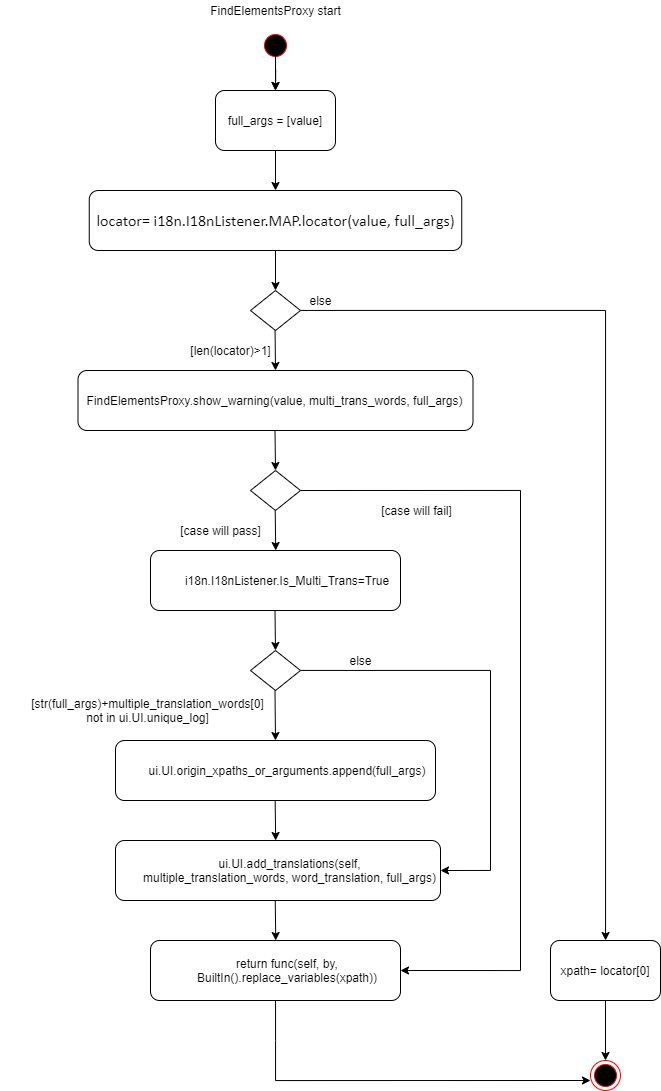
\includegraphics[width= .87\textwidth]{../UML/i18n activity diagram-FindElementsProxy.png}
    \caption{FindElementsProxy的Activity Diagram}
\end{figure}

由圖3.5 FindElementProxy的Acitivity Diagram可以得知,在新的i18n版本下,擴充一個新的代理關鍵字必須遵從著以下步驟:
\begin{itemize}
\item[1.]創出該次關鍵字呼叫的參數紀錄變數,full\_args。此變數之後會成為判斷當下待翻譯詞是否“已被使用者選擇翻譯” 的依據。並於測試腳本結束後,顯示於一詞多譯UI上,最後隨著使用者的選擇一併存入設定檔內。

\item[2.]執行翻譯。如:
\begin{lstlisting}[language={python}]
locator = i18n.I18nListener.MAP.locator(value,full_args)
\end{lstlisting}
透過i18nListener類別的MAP變數(其內裝著i18nMap類別的初始化資訊),去呼叫i18nMap類別的locator函式,對待翻譯詞value執行翻譯,且必須代入full\_args以實現1.的內容。

\item[3.]若判定此代理關鍵字遭遇一詞多譯,則產生warning資訊於報表上,如:
\begin{lstlisting}[language={python}]
FindElementsProxy.show_warning(value,multi_trans_words,full_args)
\end{lstlisting}

\item[4.]之後判斷此一詞多譯情況,最後會使測試通過或是失敗,如:
\begin{lstlisting}[language={python}]
is_actual = BuiltIn().run_keyword_and_return_status('Get WebElement', translation_locator)
if is_actual:
\end{lstlisting}

\item[5.]若測試會通過,則對預計開啟的UI做一些資料的準備,如:
\begin{lstlisting}[language={python}]
i18n.I18nListener.Is_Multi_Trans=True
if str(full_args)+multiple_translation_words[0] not in ui.UI.unique_log
ui.UI.origin_xpaths_or_arguments.append(full_args)
ui.UI.add_translations(self, multiple_translation_words, word_translation, full_args)
\end{lstlisting}
先設定再測試結束後,需要開啟一詞多譯UI。若該”參數+翻譯詞”組合尚未被翻譯過,則記錄下該次翻譯的參數部分和翻譯資訊。

\item[6.]若此次代理關鍵字沒有遭遇一詞多譯,則如:
\begin{lstlisting}[language={python}]
xpath = locator[0]
\end{lstlisting}
將第一筆翻譯同時也是唯一一筆翻譯指派給之後要回傳的xpath。

\item[7.]將翻譯好的參數部分回傳給原生的Robot Framework原生關鍵字,如:
\begin{lstlisting}[language={python}]
return func(self, by, BuiltIn().replace_variables(xpath))
\end{lstlisting}
\end{itemize}

其他未能一一介紹的代理關鍵字,儘管彼此間實作仍然存在著差異,但都是遵循著以上的架構去設計。


\hspace*{\fill} \\
\\ \hspace*{\fill} \\
\\ \hspace*{\fill} \\
\\ \hspace*{\fill} \\
\\ \hspace*{\fill} \\
\\ \hspace*{\fill} \\
\\ \hspace*{\fill} \\
\\ \hspace*{\fill} \\
%3.3
\section{改善XPath翻譯邏輯使其能應對各種html屬性}
在第一版i18n的翻譯邏輯中,若一個XPath內部存在多種html屬性,i18n工具使用了列舉法(如圖3.6),僅提供了@title、text()、normalize-space()三種屬性的翻譯規則。屆時,若測試腳本的XPath是用沒有列舉出來的屬性撰寫,但卻有翻譯的需求,例如:@placeholder、@arial-label等等,則會導致測試出錯。

\begin{figure}[H]
\begin{lstlisting}[language={python}]
default_rule = {
'((text|normalize-space)\((text\(\))?\) ?= ?(\'|\")(([0-9a-zA-Z.?&()]| )+)(\'|\"))': 4,
'((text|normalize-space)\((text\(\))?\)\, ?(\'|\")(([0-9a-zA-Z.?&()]| )+)(\'|\"))': 4,
'((@title) ?= ?(\'|\")(([0-9a-zA-Z.?&()]| )+)(\'|\"))' : 3,
'((@title), ?(\'|\")(([0-9a-zA-Z.?&()]| )+)(\'|\"))' : 3
}
\end{lstlisting}
\caption{以列舉法定義要被翻譯的HTML屬性}
\end{figure}

為了解決以上問題,本論文在多方考量下,最後採用了“負面表列法”,將確定不會執行翻譯的HTML屬性在程式中用list的方式儲存。若XPath中的HTML屬性不在該list中,則都去執行翻譯檢查。

此種作法相較於把所有HTML屬性都執行翻譯檢查,顧及到了系統執行效能,來的更加省時。相較於AI的作法,讓系統自行判斷該HTML屬性是否要翻譯,在實作上則更為簡單,且把翻譯的決定權交給了測試者,而非全部靠系統。相較於第一版i18n,把翻譯規則用列舉法固定,此作法則更能顧及到未來測試腳本的不確定性,因為我們無法預期使用者會用怎麼樣的方式去編寫XPath。

以下將以新版i18n XPath翻譯邏輯的Sequence Diagram為例(如圖3.7),輔以部分程式碼,詳述系統是如何根據當下情況,產生一套新的翻譯邏輯,以解決先前某些HTML屬性無法被翻譯的問題。

\begin{figure}[H]
    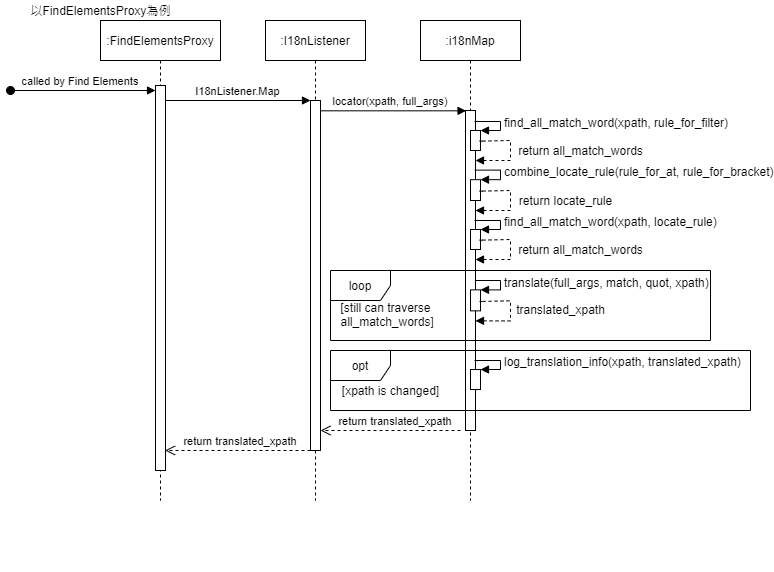
\includegraphics[width= 1.1\textwidth]{../UML/i18n sequence diagram-xpath翻譯邏輯.png}
    \caption{新版i18n XPath翻譯邏輯的Sequence Diagram}
\end{figure}

首先,FindElementsProxy會透過I18nListener呼叫I18nMap類別的locator()函式執行XPath的翻譯。之後,先定義一個內含HTML屬性特徵的rule\_for\_filter變數,如:
\begin{lstlisting}[language={python}]
rule_for_filter = {
    "(@[a-z-]*)":"@",
    "([a-z-]*\(\))":"()"
}
\end{lstlisting}
隨後呼叫find\_all\_match\_word()函式,來過濾出XPath中包含的所有屬性。

接著,先判斷這些屬性是否包含在“不需被翻譯屬性”的list中。如:
\begin{lstlisting}[language={python}]
if match not in self.no_need_trans_attirbutes:
\end{lstlisting}

若不包含其中,則根據屬性含有 ‘@’ 或 ‘()’,分別分配給rule\_for\_at和rule\_for\_bracket變數,並呼叫combine\_locate\_rule()函式,得到一套新的翻譯邏輯,locate\_rule。

之後,再次呼叫find\_all\_match\_word()函式,得到所有符合新翻譯邏輯的HTML屬性,all\_match\_words。並利用迴圈遍歷all\_match\_words中的屬性,執行translate()函式,進行翻譯檢查。
	
接著,判斷經過翻譯後,原先的xpath是否發生變化。若xpath改變,則執行log\_translation\_info()函式,將翻譯資訊顯示於測試報表上。

最後,將翻譯後的translated\_xpath,回傳給FindElementsProxy類別,完成一次XPath的翻譯。

\hspace*{\fill} \\
\\ \hspace*{\fill} \\
\\ \hspace*{\fill} \\
\\ \hspace*{\fill} \\
\\ \hspace*{\fill} \\
\\ \hspace*{\fill} \\
\\ \hspace*{\fill} \\
%3.4
\section{提供圖形化使用者介面解決一詞多譯的問題}
先前遇到一詞多譯問題時,第一版i18n工具提供了warning資訊於測試結束後的報表上,此作法確實提醒了使用者該腳本存在著一詞多譯問題,且也顯示出目前系統採用的翻譯詞,這是好的部分,本論文將繼續沿用。此翻譯邏輯是站在一個”最大化讓測試腳本通過”的立場,當遭遇一詞多譯時,系統會將所有的翻譯都執行看看,直到一包可能的翻譯中,出現了一個會使測試通過的翻譯,則算測試通過,並將該翻譯詞呈現於報表上。

然而,以上作法卻存在著一個缺陷,即是"使用者無法自由的選擇真正想要的翻譯詞"去執行腳本測試,而把決定全權授予系統。並有機會產生以下兩點問題:
\begin{itemize}
\item[1.]假如存在"多個翻譯都會使測試通過",翻譯過後的腳本測試對象,就有機會偏離使用者原先的預期。其原因可能是XPath使用contains撰寫,使得翻譯只要包含特定詞即會讓測試通過。又或是畫面上同時存在含有不同翻譯的元件,且滿足測試腳本的XPath,而導致測試通過。 
\item[2.]假如此測試腳本原先就會發生錯誤,經過翻譯後的XPath卻因為碰巧滿足畫面上的某個元件,而導致測試通過。在此特殊情形下,翻譯過後的測試對象,則更明顯的偏離了使用者原先的預期,且也改變了測試結果。 
\end{itemize}

所以,本論文將提供一個圖形化使用者介面,記錄下執行翻譯時當下的關鍵字參數組合,並顯示所有可能的翻譯詞,讓使用者從中去選擇,並產生一個設定檔,以便之後再次執行同一測試腳本時,根據設定檔的內容去選擇適當的翻譯詞。期望透過如此的方法來改善上述兩點一詞多譯所遭遇的問題。

以下,將透過圖表和Sequence Diagram的方式,來詳述一詞多譯UI的介面設計與整體實作:

一詞多譯UI的介面設計(如圖3.8),本論文將其設計成兩個區塊,上半部以條列的方式呈現完整的翻譯資訊,包含完整參數部分、待翻譯詞、可能的翻譯。下半部包含一行功能資訊的提示、一個用於開啟翻譯紀錄頁面的TransRecord按鈕,以及提交使用者選擇並寫入設定檔的Submit按鈕。
\begin{figure}[H]
    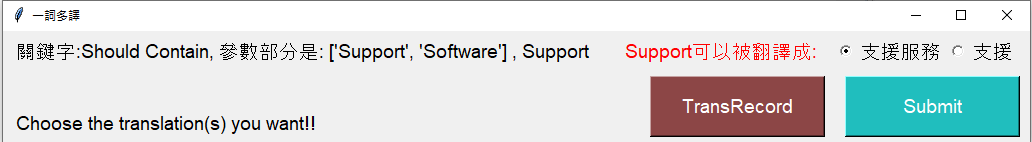
\includegraphics[width= \textwidth]{../論文截圖/3-4-1一詞多譯UI介面設計.png}
    \caption{一詞多譯UI的介面設計}
\end{figure}

翻譯紀錄的介面設計(如圖3.9),本論文同樣將其設計成兩個區塊,上半部以條列式呈現設定檔中現存的使用者翻譯選擇,下半部包含一個Undo按鈕,用於將使用者的選擇從設定檔中刪除。
\begin{figure}[H]
    \centering
    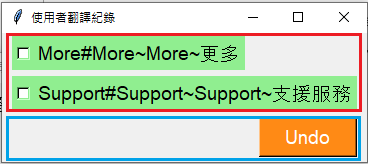
\includegraphics[width= 0.7\textwidth]{../論文截圖/3-4-2 翻譯紀錄介面設計.png}
    \caption{翻譯紀錄的介面設計}
\end{figure}

一詞多譯UI的實作,大致可以分成7個部分: run()、draw\_trans\_options()、get\_transdic\_keys\_and\_values()、open\_record()、undo\_trans()、output\_setting\_file()、\\add\_translations()。各實作彼此之間的互動關係,則如圖3.10:
\begin{figure}[H]
    \centering
    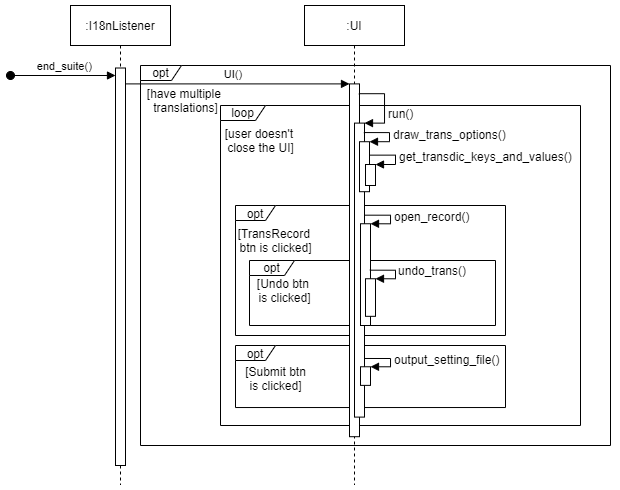
\includegraphics[width= \textwidth]{../UML/i18n sequence diagram-一詞多譯UI.png}
    \caption{產生一詞多譯UI的sequence diagram}
\end{figure}

當測試腳本結束時,會呼叫I18nListener類別的end\_suite()函式。

若本次測試腳本遭遇一詞多譯,則呼叫UI類別,使其初始化並執行run()函式,產生一詞多譯UI的介面,包含”Choose the translation(s) you want!!” 字樣、顯示翻譯紀錄的 TransRecord按鈕,以及寫入使用者選擇的Submit按鈕。之後,run()函式內部會呼叫draw\_trans\_options()函式,其內會再呼叫get\_transdic\_keys\_and\_values()函式,取出待翻譯詞與其對應的翻譯,最後隨著翻譯當下的完整參數一併顯示於一詞多譯UI的介面上。

在一詞多譯介面上,點擊TransRecord按鈕會呼叫open\_record()函式,打開翻譯紀錄介面,其會將先前使用者選擇過的翻譯詞,以條列式的方式呈現,且介面上還包含一顆Undo按鈕。點擊Undo按鈕會呼叫undo\_trans()函式,將使用者選擇的翻譯紀錄從設定檔中清除掉,同時關閉翻譯紀錄頁面。

在一詞多譯介面上,點擊Submit按鈕則會呼叫output\_setting\_file()函式,將使用者選擇的待翻譯詞對應其翻譯以及完整參數寫入設定檔”i18n/listeners/setting.txt”中,同時將剛剛已寫入的翻譯資訊從一詞多譯UI上隱藏。

此外,在UI類別中定義的add\_translations()函式,雖然不會在一詞多譯UI執行期間被呼叫,但在測試腳本執行期間,卻能負責將代理關鍵字傳入的待翻譯詞與其對應翻譯,分別儲存於變數中,方便之後get\_transdic\_keys\_and\_values()函式的讀取。並且,其還會將關鍵字的參數部分和待翻譯詞結合,成為可以辨別“該次測試腳本是否執行過相同翻譯”的字串,存入unique\_log變數中。

\hspace*{\fill} \\
\\ \hspace*{\fill} \\
\\ \hspace*{\fill} \\
\\ \hspace*{\fill} \\
\\ \hspace*{\fill} \\
%3.5
\section{將i18n工具設計成為可以安裝的模組}
本論文透過Python的build模組,將i18n工具包裝成名為”RF-AWT-i18n”的Library,並透過twine模組上傳至PYPI\cite{PYPI}網站上,使之成為可以直接讓使用者安裝的Python模組。解決了先前使用者只能從github上將i18n工具clone下來,並在該專案上開發測試腳本的不方便。

以下將詳述將i18n包裝成Python模組的步驟:

在將i18n工具打包成為一個Library前,必須先準備以下四個檔案: setup.cfg、pyproject.toml、README.md、LICENSE\cite{license}。此外必須確認將打包的資料夾下,包含\_\_init\_\_.py檔案,以被系統辨識為一個Python模組。

上述的檔案準備就緒後,便可以在i18n專案目錄下執行python –m build 指令,待建置完畢,便會產生一個名為dist的資料夾,裡面裝著打包好的RF-AWT-i18n模組檔案。接下來執行python –m twine upload –repository pypi dist/* 指令,輸入帳號密碼後,便能成功將dist資料夾中的RF-AWT-i18n模組上傳至Pypi.org網站上了。之後在PYPI網站上搜尋RF-AWT-i18n,便能看到上傳的模組。

使用者若要安裝此模組,只需執行pip install RF-AWT-i18n 指令即可(如圖3.11)。最後,使用者便可透過import此模組來使用i18n工具的功能。

\begin{figure}[H]
    \centering
    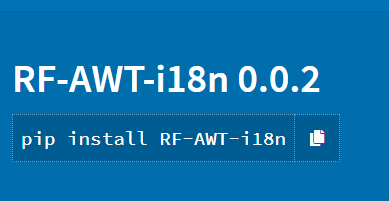
\includegraphics[width= .5\textwidth]{../論文截圖/3-5-8 安裝RF-AWT-i18n指令.png}
    \caption{安裝RF-AWT-i18n指令}
\end{figure}